For quantitative analysis, we used around 50 testing and 50 training samples of 6 classes for the face
recognition task. Each sample is re-sized to a 300x300 image. After converting each sample from color
to gray scale, we concatenated gray scale values to form a 90000 dimensional vector. We use
Principal Component Analysis to reduce the dimensions to 40 using the training dataset. Each
testing sample is also represented as 40 dimension vector as described above. We use publicly
available implementation of Wright {\em et al.}~\cite{Wright:2009:RFR:1495801.1496037}  to recognize
each input face. 

\begin{figure}
\begin{center}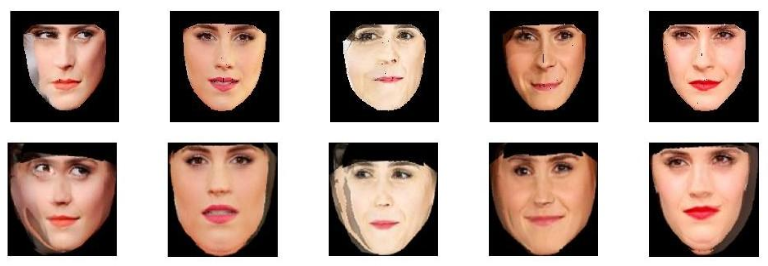
\includegraphics[width =13cm,height=5.2cm]{front/figures/qualitative_result_2.png}\end{center}
\caption{First row shows the output of our method and the second row is of Hassner {\em et al.}~\cite{DBLP:journals/corr/HassnerHPE14} for PIWFDS dataset.}
\label{fig:qualitative_result2}
\end{figure}

Accuracy is calculated as fraction of testing samples classified correctly over the total number of samples. Our method achieved an accuracy of 31\%, which is significantly better than 27\% achieved by Hassner {\em et al.}.
